\documentclass[12pt]{article}
\usepackage[utf8]{inputenc}
\usepackage{graphicx} % Allows you to insert figures
\usepackage{amsmath} % Allows you to do equations
\usepackage{fancyhdr} % Formats the header
\usepackage{geometry} % Formats the paper size, orientation, and margins
\usepackage[style=authoryear-ibid,backend=biber]{biblatex} % Allows you to do citations - does Harvard style and compatible with Zotero
\addbibresource{Example.bib} % Tells LaTeX where the citations are coming from. This is imported from Zotero
\usepackage[english]{babel}
\usepackage{csquotes}
\usepackage{background}
\usepackage{minted}
\renewcommand*{\nameyeardelim}{\addcomma\space} % Adds comma in in-text citations
\linespread{1.5} % About 1.5 spacing in Word
\setlength{\parindent}{0pt} % No paragraph indents
\setlength{\parskip}{1em} % Paragraphs separated by one line
\renewcommand{\headrulewidth}{0pt} % Removes line in header
\geometry{a4paper, portrait, margin=1in}
\setlength{\headheight}{14.49998pt}
\backgroundsetup{scale=1,angle=0,opacity=0.175,contents={
\includegraphics[scale=0.25]{1200px-Vellore_Institute_of_Technology_seal_2017.png}}}


\begin{document}
\begin{titlepage}
\NoBgThispage
   \begin{center}
        \begin{figure}[h] % h - Place the float here, i.e., approximately at the same point it occurs in the source text (however, not exactly at the spot)
        \centering
        
\includegraphics[width=15cm]{1583124354phpJTtnK5.png}
        \end{figure}

        \Huge{Digital Assignment 3}

        \vspace{0.5cm}
        \LARGE{20BIT0380 - Hardik Nagpal\\20BIT0386 - Raghav Gupta\\20BIT0381 - Niladri Mitra\\20BIT0406 - Sanchit Sandeep Khedkar\\20BIT0015 - Atishay Jain}
       
        \vspace{2.5 cm}
        \Large{2022-04-21}
        
        \vspace{0.25 cm}
        \Large{ITE2015 - Information Systems Audit}
        \large{VL2021220502557}
       

       \vfill
    \end{center}
\end{titlepage}
\newpage
1. Describe the purposes of long-run planning in relation to the information systems audit function. Also explain how might the nature and extent of long run planning for the information systems audit function differ depending upon where an organization is placed\\
When we undertake long-run planning in relation to the information systems audit function, our purposes are twofold:\\ 
(1) to provide an overall direction for the function and\\ 
(2) to try to ensure we will have adequate resources to discharge the responsibilities associated with the function effectively and efficiently. Our determination of the former goal will have a marked influence on our deliberations in relation to the latter goal.\\\\
The purpose of long run planning is to help an organization establish priorities to better meet its mission. This planning encompasses an organization’s leadership, organizational structures and processes. This planning can help ensure that the organization achieves its strategic goals and objectives. An organization’s environment must be aligned with its long-run strategic plan, goals and objectives.Long run planning allows an organization to collaboratively align with its mission in a high-quality, meaningful way in order to create a strategic vision of what the organization is, what it wants to be, and how it can change with times. Basically, long run planning helps an organization project its desired future. An organization’s mission is its purpose and reason for being. It serves as a guiding light. \\\\
Overall, the long-run goal of the information systems audit function should be to support the mission of the organization in which it is placed. We must determine, therefore, how critical the goals of asset safeguarding, data integrity, system effectiveness, and system efficiency are to the host organization. Clearly, these four goals will be important to some extent in all organizations. We must recognize, however, that their relative importance will vary across organizations. For example, asset safeguarding and data integrity are likely to be of paramount importance to financial institutions. In a consulting firm, however, asset safeguarding and data integrity often will be a minor concern. The firm is likely to have few information systems assets to safeguard and little data that is critical to its operations.\\\\
In the context of the information systems audit function, we would expect that asset safeguarding, data integrity, effectiveness, and efficiency will become more critical as the importance of existing and future information systems to an organization increases. Accordingly, we will need to undertake more planning in relation to the information systems audit function. Similarly, as the importance of future information systems to an organization increases, we will need to undertake more long-run planning in relation to the information systems audit function.\\\\
We must recognize, also, that it might be possible to turn the goals of asset safeguarding, data integrity, effectiveness, and efficiency into a source of competitive advantage for an organization. In this light, planning for the information systems audit function should not always the secondary to the overall planning undertaken on the organization's mission and goals. In some organizations, it might be possible to use the activities of the information systems audit function to affect the determination of the organization's mission and goals. To the extent that the information systems audit function allows new levels of asset safeguarding, data integrity, effectiveness, and efficiency to be achieved, the organization might be able to undertake strategic initiatives for example, that lead it to compete in new mark.\\\\
We need to adapt a contingency perspective on the nature of and amount of long-run planning we undertake in relation to the information systems audit function. In this regard, strategic grid might help us make this determination.They focus on the importance of existing information systems and the importance of future information systems in determining the nature of and extent of information systems planning that should be undertaken within an organization. The extent of planning needs to increase as the importance of existing and future information systems to an organization increases. Similarly, more long-run planning needs to be undertaken as the importance of future information systems to an organization increases.The organization placed means that the organization is located in various places, it has many branches , its main office is somewhere and its other office is somewhere . So as in this case we already discussed one branch might focus on some other goal whereas main branch i.e HeadOffice will focus on achieving all the goals , while for a branch that belongs to consulting only for them safeguarding and data integrity often will be a minor concern. So in this way as discussed above the Nature and extent of long run planning differ depending on where organization is placed\\\\
\begin{figure}[h] % h - Place the float here, i.e., approximately at the same point it occurs in the source text (however, not exactly at the spot)
\begin{subfigure}
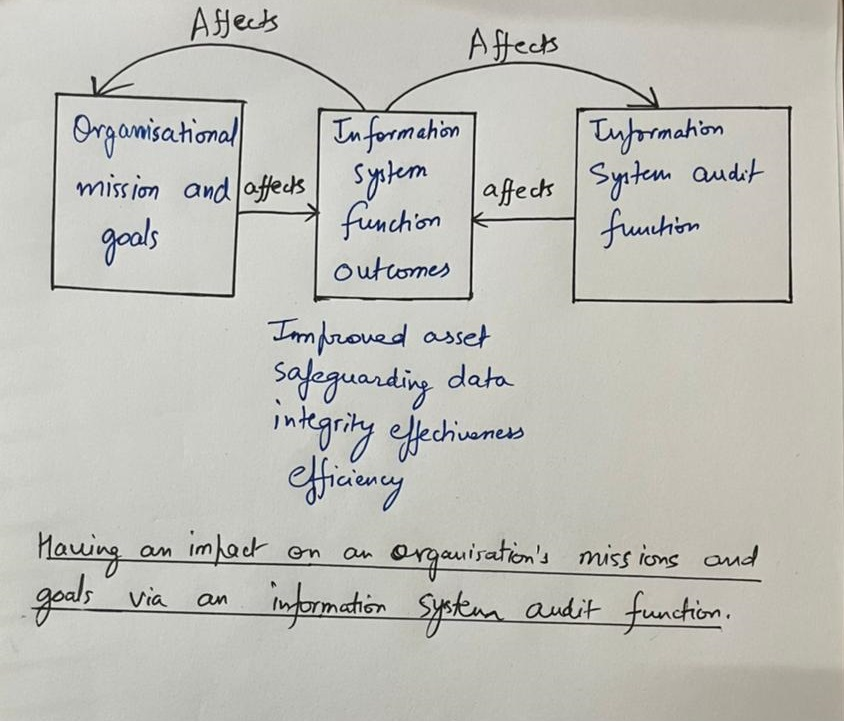
\includegraphics[scale=0.5]{1.jpeg}
\end{subfigure}
\begin{subfigure} % h - Place the float here, i.e., approximately at the same point it occurs in the source text (however, not exactly at the spot)
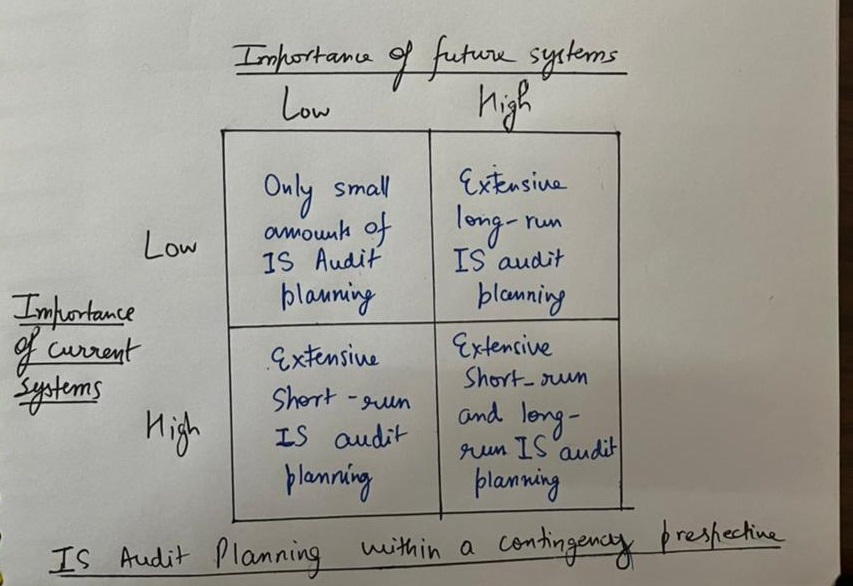
\includegraphics[scale=0.5]{2.jpeg}
\end{subfigure}
\end{figure}
\newpage
\newpage
2. Why might auditors have to use surrogate measures to assess the impact of an information system on the quality of working life of its users? Give three surrogate measures that auditors might employ and explain briefly how they might be useful.\\
To evaluate the impact of an information system on users' quality of working life, auditors may look for proxies or surrogate measures of the impact. Surrogate measures act as indicators of the quality of work life existing instead of directly measuring attributes of the quality of working life.\\There are three advantages of using surrogate measures to assess the quality of working life.\\First, the measures are objective, verifiable, and difficult to manipulate. If auditors can obtain agreement among stakeholders that they are reasonable indicators of the quality-of-working-life changes that are associated with an information system, they are not likely to then encounter problems with disputes about their accuracy and reliability.\\Second, the data required for the measures is relatively easy to obtain. Most of the data should be maintained routinely by an organisation. For example, the personnel department of the organisation should keep records on sickness, absenteeism, and strikes.\\Third, the cost of changes in the measures can be assessed. For example, absenteeism can be measured by calculating the cost of wages and fringe benefits of replacement workers, the opportunity cost of profit-loss during the replacement process and the cost of the personnel department's time in dealing with absenteeism.\\The major disadvantage of using surrogate measures is that auditors will not always know why the quality of working life has been lowered or raised by an information system. What attributes of the quality of the working life have been affected by the implementation of a system still must be determined. Otherwise, if the quality of working life has been lowered, there's little basis for corrective  action. Use of surrogate measures does not alleviate an auditor's need, therefore, to investicate cause-effect relationships.\\Some surrogate measures are as follows-\[Absenteeism\hspace{0.15cm} Rate=\frac{total\hspace{0.2 cm}absent\hspace{0.2cm}days}{total\hspace{0.2cm}working\hspace{0.2cm} days}\]\[Strike\hspace{0.15cm} Rate=\frac{total\hspace{0.2cm} strike\hspace{0.2cm} days}{total\hspace{0.2cm} working\hspace{0.2cm} days}\]\[Turnover\hspace{0.15cm} Rate=\frac{total\hspace{0.2cm} turnover\hspace{0.2cm} incidents}{average\hspace{0.2cm} working\hspace{0.2cm} force\hspace{0.2cm} size}\]A lowered quality of working life may lead to increased increased turnover of employees, or increased absenteeism, or greater number of strikes. Thus to assess the effectiveness of the impact of an information system on quality of working life, the focus is on how these measures change after the system has been implemented.
\end{document}
